\documentclass[11pt,aspectratio=169,handout]{beamer}
%
%\usetheme{Singapore}
%\usecolortheme{orchid}

\usepackage[utf8]{inputenc}
\usepackage[russian]{babel}
\usepackage{amsmath}
\usepackage{amsfonts}
\usepackage{amssymb}
\usepackage{graphicx}
\usepackage{bibentry}
\usepackage{wasysym}
\usepackage[most]{tcolorbox}
\usepackage[normalem]{ulem}

\usepackage{hyperref}

\definecolor{info}{RGB}{62, 180, 137}
\definecolor{warn}{RGB}{128, 0, 0}
\definecolor{vk}{RGB}{51, 117, 246}

\usepackage{fontspec}
\setsansfont{VK Sans Display}

\setbeamercolor{frametitle}{fg=vk}
\setbeamercolor{title}{fg=vk}
\setbeamerfont{frametitle}{size=\LARGE}
\setbeamerfont{title}{size=\LARGE}
\addtobeamertemplate{frametitle}{\vspace*{0.5em}\hspace*{1em}}

\useinnertheme{circles}

\setbeamertemplate{title page}[default][left]


\author{\hspace{-0.5cm} Николай Анохин}
\title{\hspace{-0.55cm} Рекомендательные системы}
\date{}

%\logo{\includegraphics[width=.05\textwidth]{images/ok_logo.png}}

\AtBeginSection[]{
  \begin{frame}
  \vfill
  \centering
  \begin{beamercolorbox}[sep=8pt,center,shadow=true,rounded=true]{title}
    \usebeamerfont{title}\insertsectionhead\par
  \end{beamercolorbox}
  \vfill
  \end{frame}
}

\begin{document}

{
\setbeamertemplate{headline}{}

{
\usebackgroundtemplate{
\includegraphics[width=\paperwidth]{images/title.png}}
\begin{frame}[b]
\vfill
\titlepage
\end{frame}
}

%\begin{frame}
%\tableofcontents
%\end{frame}

}

\section{Информация о курсе}

%\begin{frame}{Входной опрос}
%
%\begin{columns}
%
%\begin{column}{0.45\textwidth}
%   \begin{center}
%   \includegraphics[scale=0.4]{images/please.jpeg}
%   \end{center}
%\end{column}
%
%\begin{column}{0.45\textwidth}
%  \begin{center}
%  \includegraphics[scale=0.1]{images/survey.png}
%  \end{center}
%\end{column}
%
%\end{columns}
%
%\begin{center}
%\url{https://shorturl.at/aUrOo}
%\end{center}
%
%\end{frame}

\begin{frame}{Николай Анохин}

\begin{center}
\includegraphics[scale=0.23]{images/about-me.png}
\end{center}

\end{frame}

\begin{frame}{Олег Сапрыкин}

\begin{center}
\includegraphics[scale=0.32]{images/about-me-oleg.png}
\end{center}

\end{frame}

\begin{frame}{Евгений Кувшинов}

\begin{center}
%\includegraphics[scale=0.32]{images/about-me-oleg.png}
\end{center}

\end{frame}

\begin{frame}{Маргарита Маркова}

\begin{center}
%\includegraphics[scale=0.32]{images/about-me-oleg.png}
\end{center}

\end{frame}

\begin{frame}{Сергей Малышев}

\begin{center}
\includegraphics[scale=0.32]{images/about-me-sergey.png}
\end{center}

\end{frame}

\begin{frame}{Роман Логойда}

\begin{center}
%\includegraphics[scale=0.32]{images/about-me-oleg.png}
\end{center}

\end{frame}

\begin{frame}{Как задать вопрос}

\begin{itemize}
\item Голосом
\item В специально выделенное для этого время
\item Перед тем как спросить будет хорошим тоном поставить несколько знаков вопроса
\begin{tcolorbox}[colback=gray!5,colframe=gray!80,title=]
20:23 Саша: ???? \\
20:23 Преподаватель: Ждём вопроса от Саши \\
20:24 Саша: Какая метрика хорошо работает в задаче рекомендаций?
\end{tcolorbox}
\end{itemize}

\end{frame}

\begin{frame}{Если что-то пошло не так}

\begin{itemize}
\item Пропал голос
\item Исчезло изображение
\item Плохо слышно
\item Любые проблемы другого характера
\end{itemize}
\vfill
{\bf Сразу пишем в чат} много минусов и не ждем других участников. Если вы увидели, что в чате кто-то написал много минусов, а у вас всё хорошо, то поставьте несколько плюсов:
\vfill
\begin{tcolorbox}[colback=gray!5,colframe=gray!80,title=]
20:24 Петя: - - - - - - -  \\
20:25 Саша: ++++ \\
20:25 Ольга: +++++++
\end{tcolorbox}

\end{frame}

\begin{frame}{Пройдя этот курс, вы...}

\begin{itemize}
\item Разработаете свой рекомендательный сервис (почти) с нуля
\item Сможете выбирать правильные инструменты под конкретную задачу
\item Узнаете о проблемах, возникающих в боевых RS, и научитесь их решать
\item Будете в курсе SOTA моделей и задач RS, над которыми работают ученые
\item Подготовитесь к собеседованию по RS на junior позицию
\end{itemize}

\end{frame}

{
\usebackgroundtemplate{\includegraphics[width=\paperwidth]{images/mle.png}}
\begin{frame}[plain]
\end{frame}
}

\begin{frame}{}

Репозиторий: \url{https://github.com/anokhin/recsys-course-spring-2026}

Чат курса: \url{TODO}

\vfill

\begin{itemize}
\item Вопросы вне занятия можно задать в личке или в чате курса (лучше)
\item Тегайте нас, чтобы мы не пропустили ваш комментарий в общем потоке сообщений
\item Если ответа не последовало в течении 24 часов, то мы, вероятно, не увидели ваше сообщение. Не стесняйтесь его продублировать
\end{itemize}

\end{frame}

\section{Краткий обзор рекомендательных систем}

\begin{frame}{}

\vfill
\begin{tcolorbox}[colback=info!5,colframe=info!80,title=]
{\bf Recommender Systems} (RS) are software tools and techniques providing suggestions for {\bf items} to be of use to a {\bf user} \cite{RSHB}.
\end{tcolorbox}
\vfill
\begin{center}
\includegraphics[scale=0.3]{images/overall.png}
\end{center}

\end{frame}

{
\usebackgroundtemplate{\includegraphics[width=\paperwidth, height=\paperheight]{images/netflix-0.png}}
\begin{frame}[plain]
\end{frame}
}

{
\usebackgroundtemplate{\includegraphics[width=\paperwidth, height=\paperheight]{images/netflix-6.png}}
\begin{frame}[plain]
\end{frame}
}

\begin{frame}{RS в индустрии и науке}

{\bf Компании}

Amazon.com, YouTube, Netflix, Yahoo, Tripadvisor, Spotify, Booking.com

\vfill

{\bf Конференции}

RecSys, KDD, WSDM, SIGIR

\vfill

{\bf Книги}

Recommender Systems Handbook \cite{RSHB}, Mining of Massive datasets \cite{MMDS}

\end{frame}

\begin{frame}{RS vs другие задачи ML \cite{NETFLIX}}

\begin{itemize}[<+->]
\item RS ориентированы на продакшен
\item Наблюдаемые данные очень разреженные
\item Отсутствующие данные -- missing not-at-random
\item Отсутствующие данные -- либо ненаблюдаемые позитивные, либо негативные
\item Рекомендательные сервисы живут в петле обратной связи
\end{itemize}

\end{frame}

\begin{frame}{Зачем RS бизнесу}

\begin{columns}

\begin{column}{0.45\textwidth}
   \begin{small}
    \begin{itemize}[<+->]
	\item Увеличить продажи
	\item Продвигать более разнообразные айтемы
	\item Улучшить пользовательский опыт
	\item Добиться большей лояльности
	\item Лучше понимать пользователей
	\end{itemize}
    \end{small}
\end{column}

\begin{column}{0.45\textwidth}
   \begin{center}
		\includegraphics[scale=0.25]{images/logos-en.png}
   \end{center}
\end{column}

\end{columns}

\end{frame}

\begin{frame}{Зачем RS пользователям}

\begin{columns}

\begin{column}{0.45\textwidth}
   \begin{small}
    \begin{itemize}[<+->]
	\item Найти лучший товар
	\item Найти {\bf все} подходящие товары
	\item Найти последовательность или набор товаров
	\item Залипнуть
	\end{itemize}
    \end{small}
\end{column}

\begin{column}{0.45\textwidth}
   \begin{center}
		\includegraphics[scale=0.25]{images/logos-ru.png}
   \end{center}
\end{column}

\end{columns}

\end{frame}

\begin{frame}{Зачем RS инженерам}

\begin{columns}
\begin{column}{0.4\textwidth}
   \begin{center}
                \includegraphics[scale=0.25]{images/computerdog.jpeg}
   \end{center}
\end{column}
\begin{column}{0.5\textwidth}
    \begin{small}
    \begin{itemize}
    \item Делать высоконагруженный отказоустойчивый сервис :D
    \item Анализировать большие данные
    \item Окунуться в волшебный мир \sout{матана} машинного обучения
    \item Объективно измерять результат своей работы 
    \item Узнать много нового о людях
    \item Все это за зарплату
    \end{itemize}
    \end{small}
\end{column}
\end{columns}

\end{frame}

%--------------------------------------------------

\begin{frame}{Обзор типичных компонентов RS / \\ Mendeley (2016) \cite{MNDL}}
% Components
\begin{columns}
\begin{column}{0.6\textwidth}
   \begin{center}
		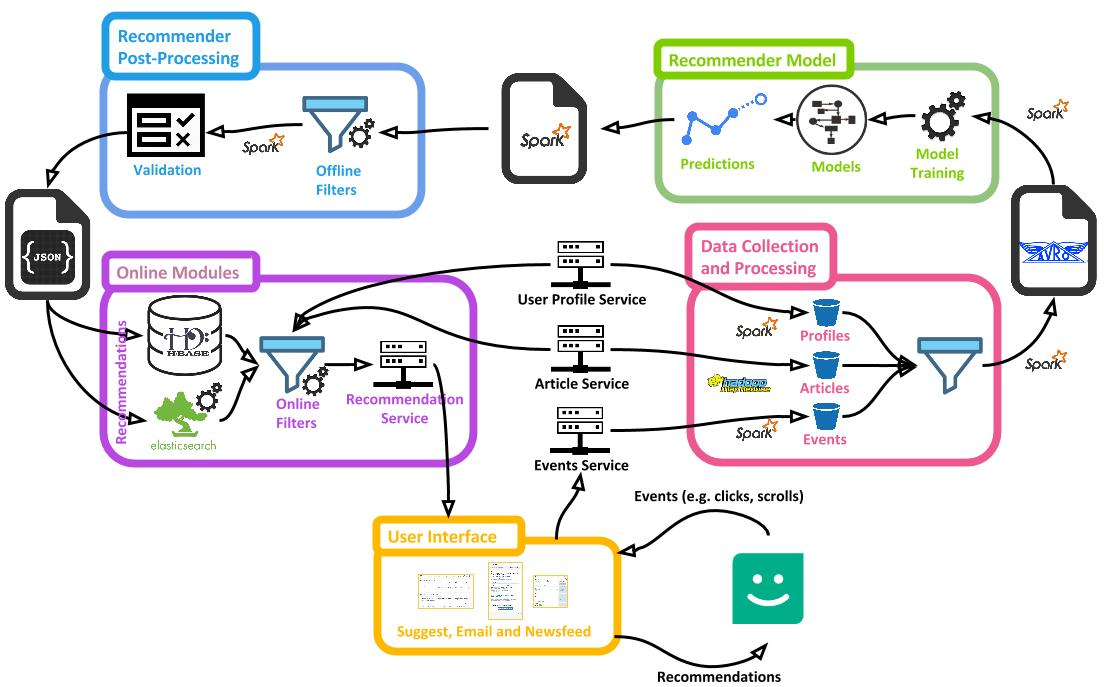
\includegraphics[scale=0.2]{images/mendeley.jpeg}
   \end{center}
\end{column}
\begin{column}{0.35\textwidth}
    \begin{tcolorbox}[colback=info!5,colframe=info!80,title=]
    \begin{small}
    Машинное обучение -- небольшая часть рекомендательного сервиса. Другие компоненты часто требуют не меньше усилий.
    \end{small}
    \end{tcolorbox}
\end{column}
\end{columns}

\footnote{Ссылки:
\href{https://hadoop.apache.org/}{Hadoop} +
\href{https://spark.apache.org/}{Spark} +
\href{https://hbase.apache.org/}{HBase} +
\href{https://www.elastic.co/what-is/elasticsearch}{Elasticsearch}
}

\end{frame}

%--------------------------------------------------

\begin{frame}{Рекомендации айтемов из больших каталогов / Youtube (2016) \cite{YTBE}}
% Enormous action space, context
\begin{columns}
\begin{column}{0.6\textwidth}
   \begin{center}
		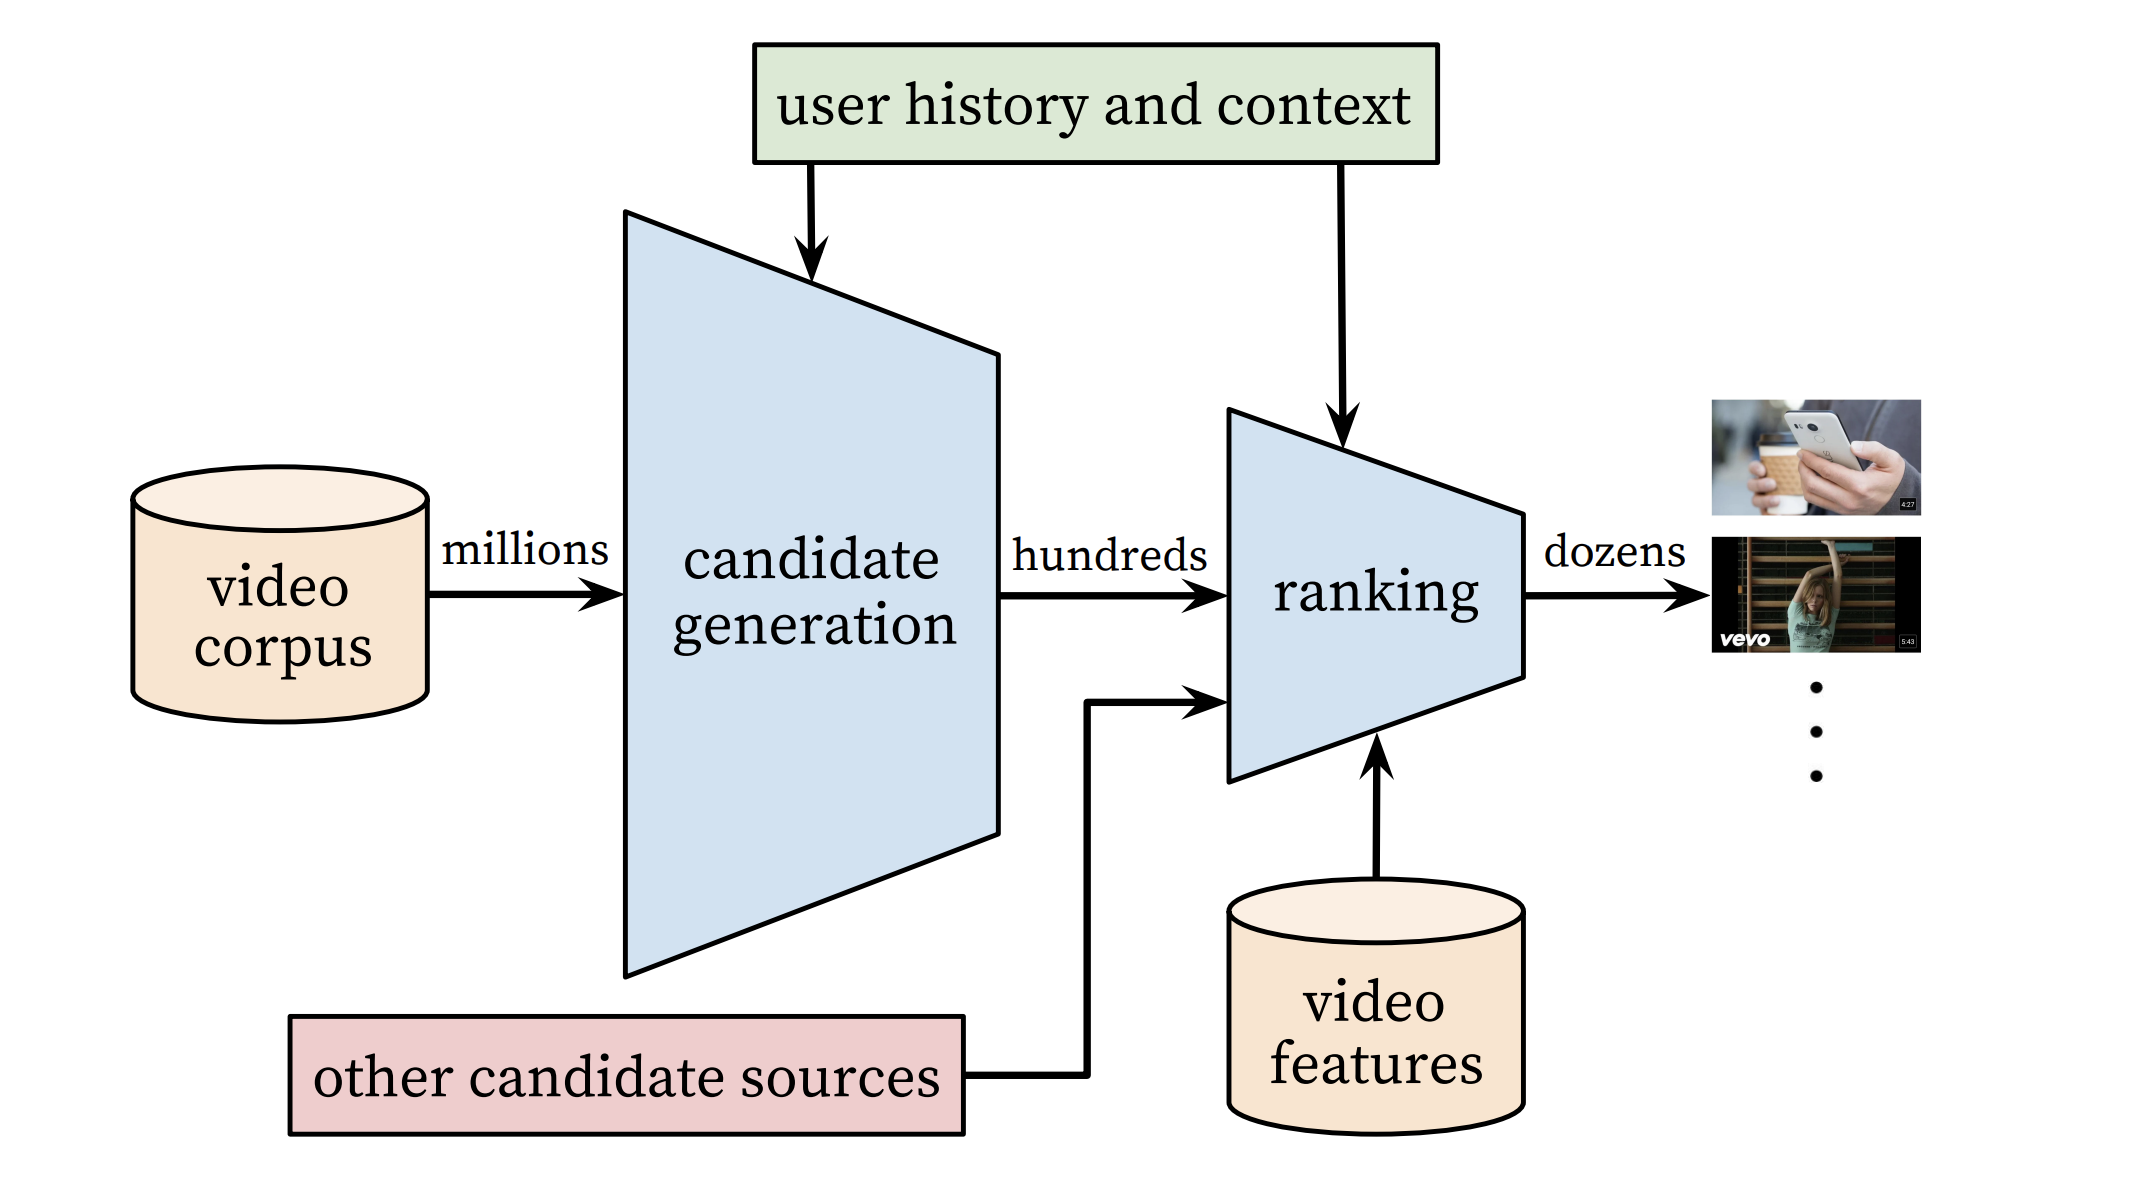
\includegraphics[scale=0.25]{images/youtube.png}
   \end{center}
\end{column}
\begin{column}{0.35\textwidth}
   \begin{small}
    \begin{tcolorbox}[colback=info!5,colframe=info!80,title=]
    Айтемов так много, что учесть {\bf полный контекст} не может даже Google. Для быстрого отбора кандидатов применяются грубые фильтры.
    \end{tcolorbox}
    \end{small}
\end{column}
\end{columns}

\end{frame}

%--------------------------------------------------

\begin{frame}{Уровни вычислений и двухэтапный рекомендер \cite{YAN}}

\begin{center}
	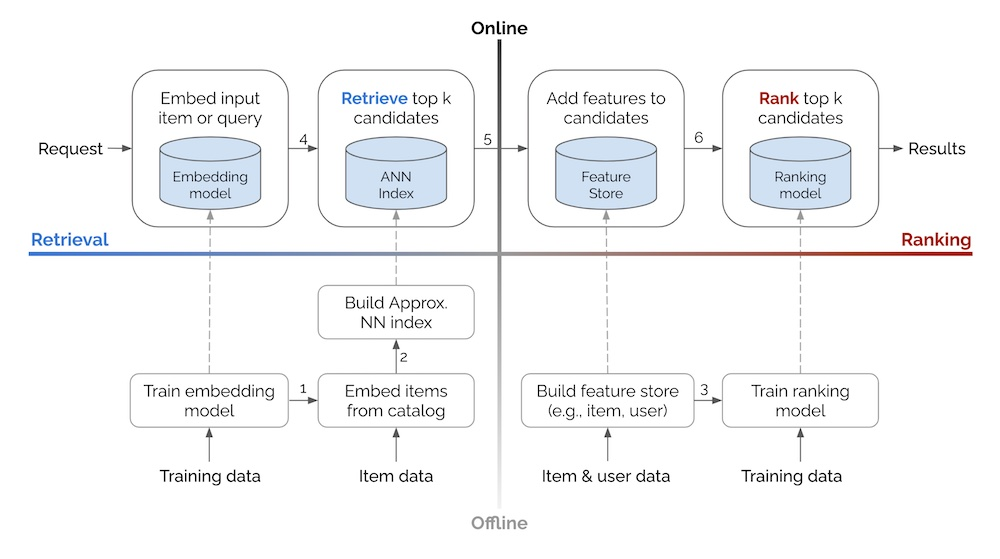
\includegraphics[scale=0.3]{images/discovery-system-design.jpg}
\end{center}

\end{frame}

%--------------------------------------------------

\begin{frame}{Как выбрать техническую метрику}

\begin{columns}
\begin{column}{0.55\textwidth}
   \begin{center}
     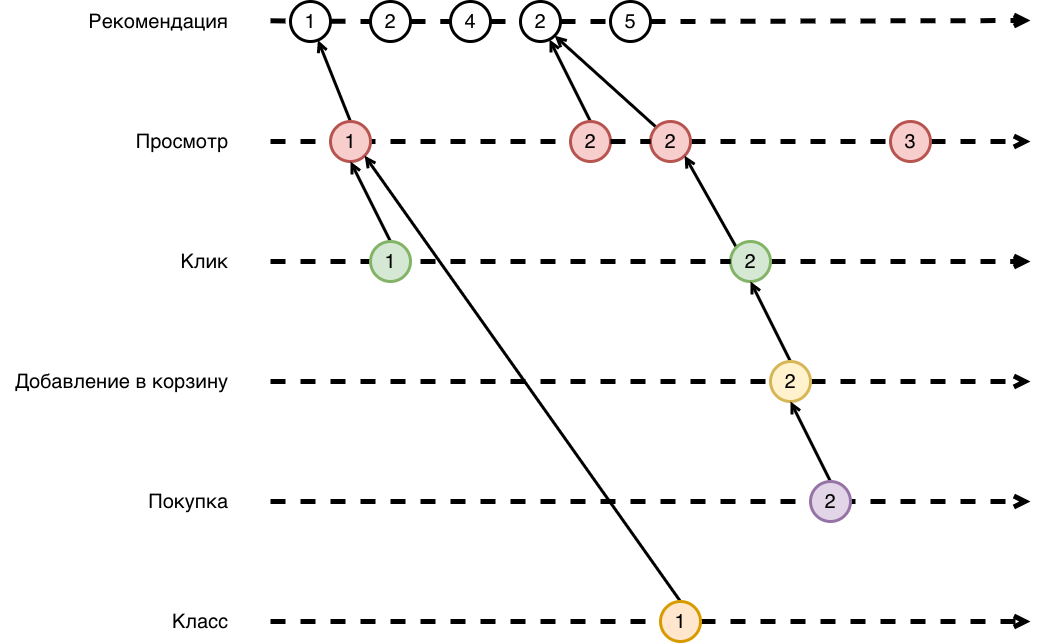
\includegraphics[scale=0.17]{images/recommendation-events.png}
  \end{center}
\end{column}
\begin{column}{0.4\textwidth}
    \begin{tcolorbox}[colback=gray!5,colframe=gray!80,title=фидбэк на рекомендации]
    \begin{itemize}%[<+->]
    \item[-] Явный/explicit
    \item[-] Неявный/implicit
    \item[-] Отложенный/delayed
    \end{itemize}
    \end{tcolorbox}
\end{column}
\end{columns}

\vfill

Какие пользовательские данные использовать для метрики?
\begin{itemize}
\item События, интересные бизнесу: их мало и долго ждать
\item Быстрые события: их много, но они хуже отражают задачу
\end{itemize}

\end{frame}

%--------------------------------------------------

\begin{frame}

\begin{footnotesize}

\begin{center}

\begin{tabular}{l c c c c c}
Цель & rel & cov & div & ser & poll \\
\hline
{\bf Бизнесу} & & & & & \\
\hline
Увеличить продажи & \checked & & & \checked & \\
Продвигать более разнообразные айтемы & & \checked & \checked & & \\
Улучшить пользовательский опыт & \checked & & \checked & \checked & \checked \\
Добиться большей лояльности & & & & & \checked \\
Лучше понимать пользователей & & & & & \checked \\
\hline
{\bf Пользователям} & & & & & \\
\hline
Найти лучший товар & \checked & & & \checked & \checked \\
Найти {\bf все} подходящие товары & \checked & \checked & & & \checked \\
Найти последовательность или набор товаров & \checked & & & \checked & \checked \\
Залипнуть & \checked & & \checked & \checked & \checked \\
\end{tabular}

\end{center}

\end{footnotesize}

\end{frame}

%--------------------------------------------------

\begin{frame}{Precision@k, Recall@k}

\begin{columns}
\begin{column}{0.5\textwidth}
   \begin{tcolorbox}[colback=gray!5,colframe=gray!80,title=]
\[
      Precision@k = \frac{no.\ relevant\ items}{k}\\
\]
\[
      Recall@k = \frac{no.\ relevant\ items\ in\ k}{total\ no.\ relevant\ items}\\
\]
   \end{tcolorbox}
   \begin{center}
		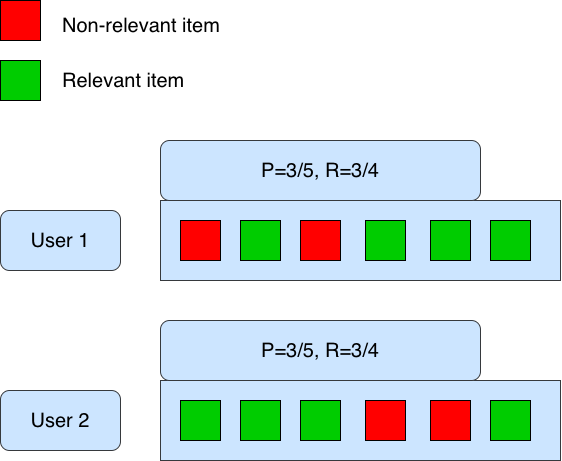
\includegraphics[scale=0.22]{images/precision-recall.png}
   \end{center}
\end{column}
\begin{column}{0.4\textwidth}
    \begin{tcolorbox}[colback=info!5,colframe=info!80,title=]
      \begin{itemize}
      \item Легко интерпретировать
      \item Легко реализовать
      \end{itemize}
    \end{tcolorbox}
    \begin{tcolorbox}[colback=warn!5,colframe=warn!80,title=]
      \begin{itemize}
      \item Нечувствительны к порядку внутри $k$
      \item Не дают общей картины для любого $k$
      \end{itemize}
    \end{tcolorbox}
\end{column}
\end{columns}

\end{frame}

%--------------------------------------------------

\begin{frame}{Normalized Discounted Cumulative Gain}

\begin{columns}
\begin{column}{0.5\textwidth}
   \begin{center}
		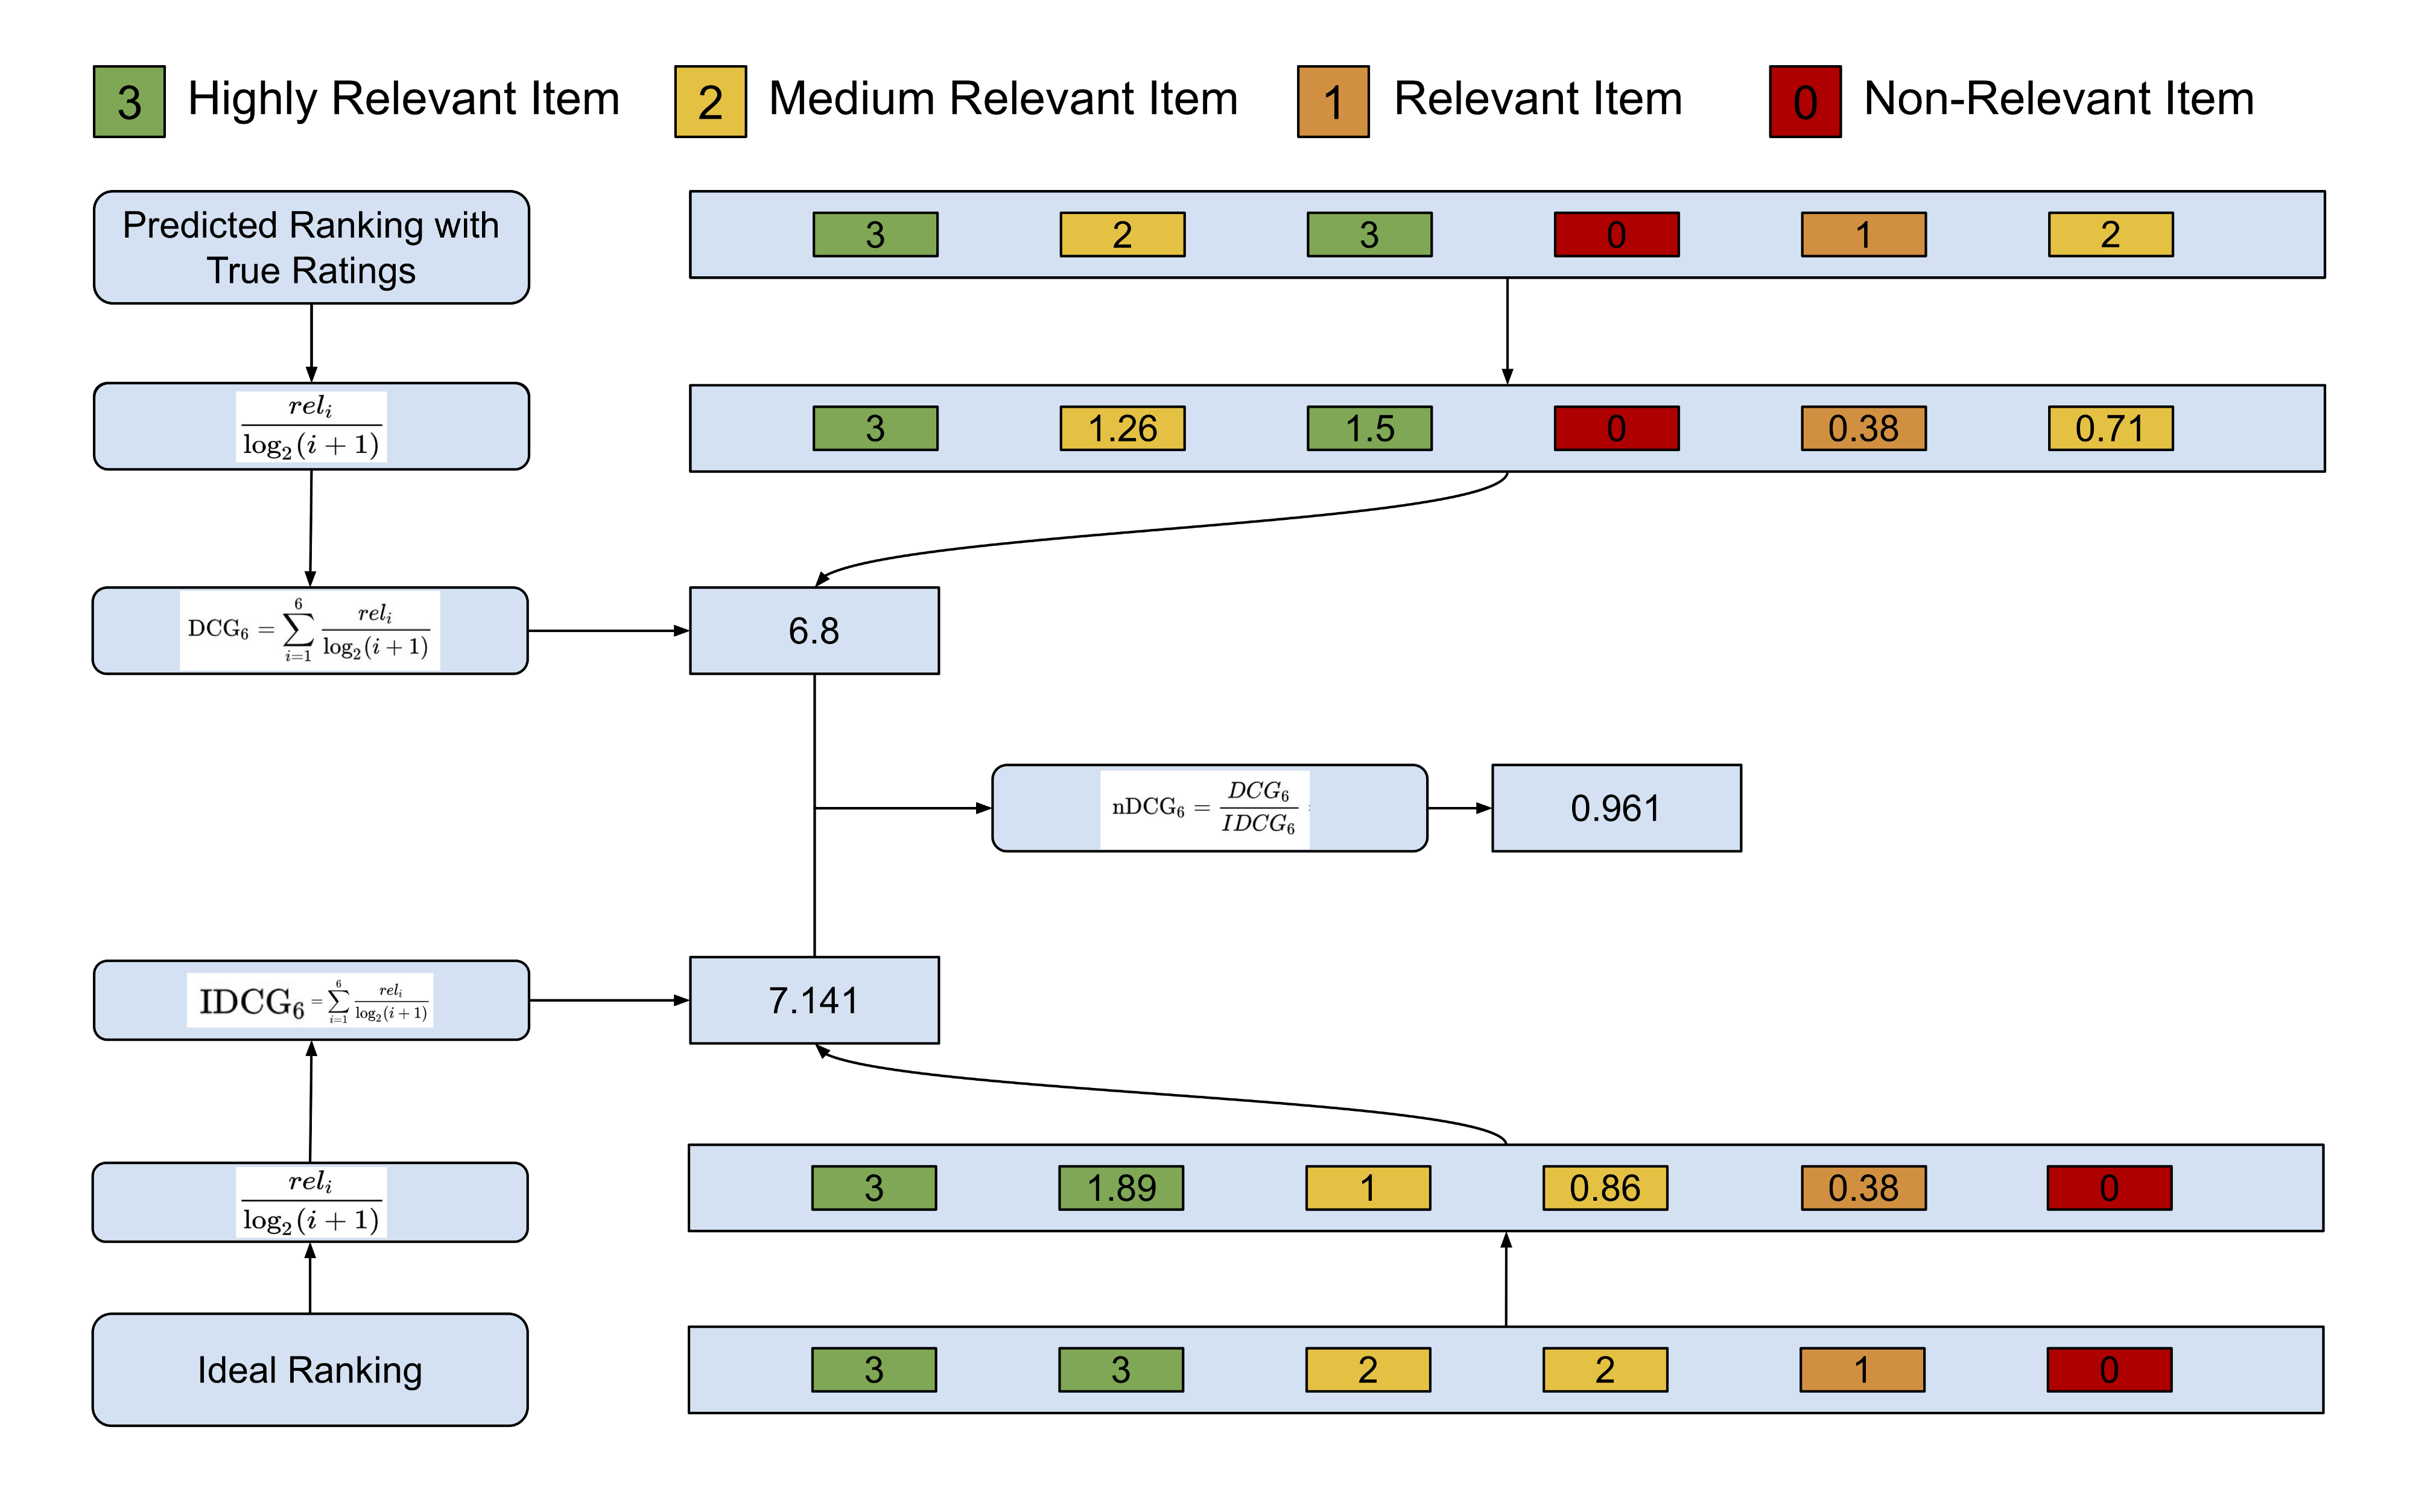
\includegraphics[scale=0.055]{images/ndcg.png}
   \end{center}
\end{column}
\begin{column}{0.4\textwidth}
    \begin{tcolorbox}[colback=info!5,colframe=info!80,title=]
      \begin{itemize}
      \item Учитывает не только бинарный фидбэк
      \item Хорошо учитывает позицию
      \end{itemize}
    \end{tcolorbox}
    \begin{tcolorbox}[colback=warn!5,colframe=warn!80,title=]
      \begin{itemize}
      \item Сложно интерпретировать
      \end{itemize}
    \end{tcolorbox}
\end{column}
\end{columns}

\end{frame}

%--------------------------------------------------

\begin{frame}

\begin{columns}

\begin{column}{0.47\textwidth} 

\begin{center}
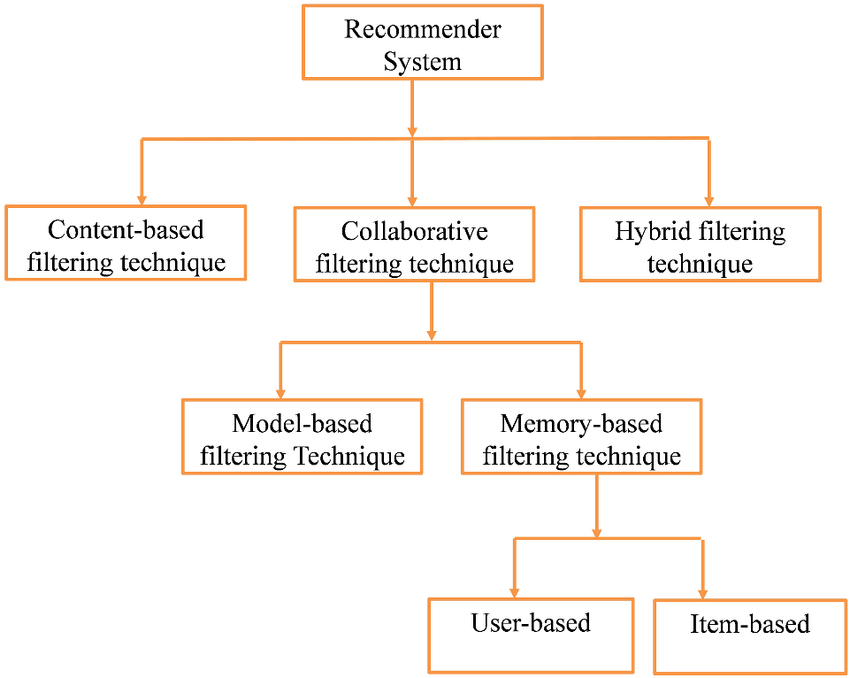
\includegraphics[scale=0.22]{images/taxonomy.png}
\end{center}

\end{column}

\begin{column}{0.47\textwidth} 

\begin{center}

\includegraphics[scale=0.2]{images/karlson.png}
\end{center}

\end{column}

\end{columns}

\end{frame}

%--------------------------------------------------

\begin{frame}{Content-based RS}

\begin{columns}

\begin{column}{0.47\textwidth} 
\begin{tcolorbox}[colback=info!5,colframe=info!80,title=Идея]
Рекомендуем пользователю айтемы, похожие на те, что нравились ей раньше
\end{tcolorbox}
\end{column}

\begin{column}{0.47\textwidth} 
\begin{center}
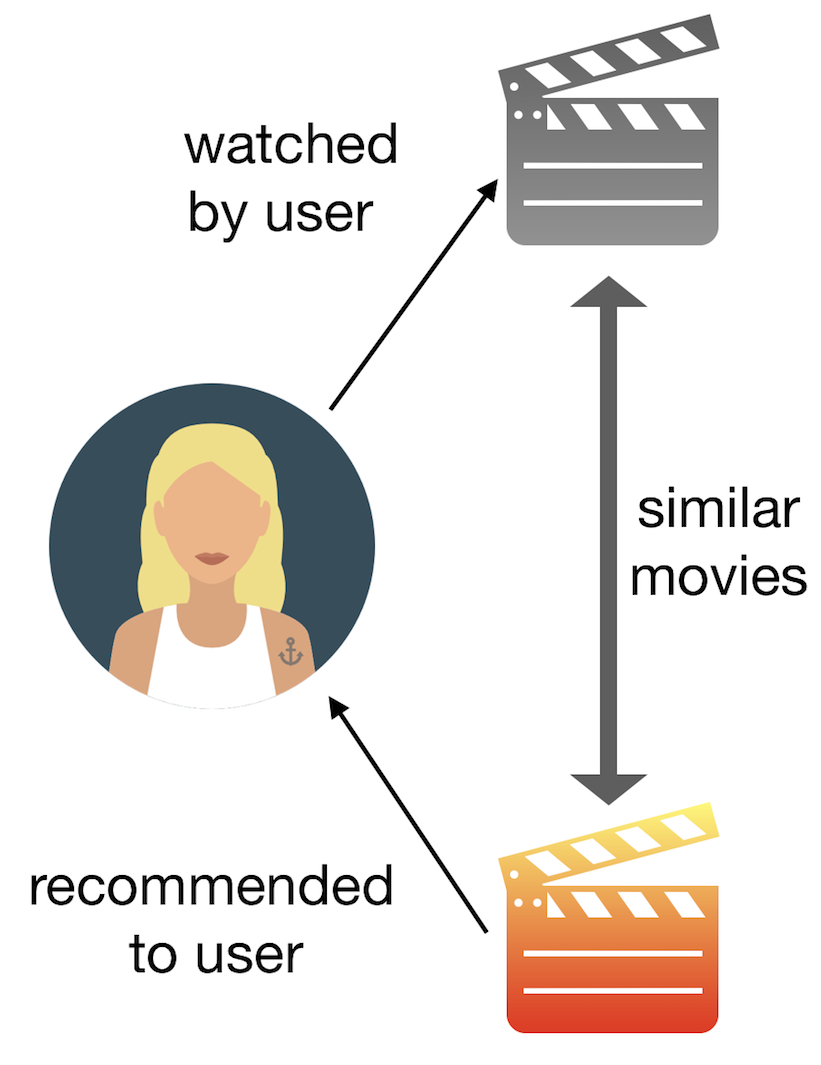
\includegraphics[scale=0.15]{images/content-idea.png}
\end{center}
\end{column}

\end{columns}

\end{frame}

%--------------------------------------------------

\begin{frame}{Collaborative filtering\footnote{Оскар за худшее название алгоритма}-based RS}

\begin{columns}

\begin{column}{0.47\textwidth} 
\begin{tcolorbox}[colback=info!5,colframe=info!80,title=Идея]
Рекомендуем пользователю айтемы, которые понравились похожим на нее пользователям. Пользователи похожи, если они похоже оценивают одни и те же айтемы.
\end{tcolorbox}
\end{column}

\begin{column}{0.47\textwidth} 
\begin{center}
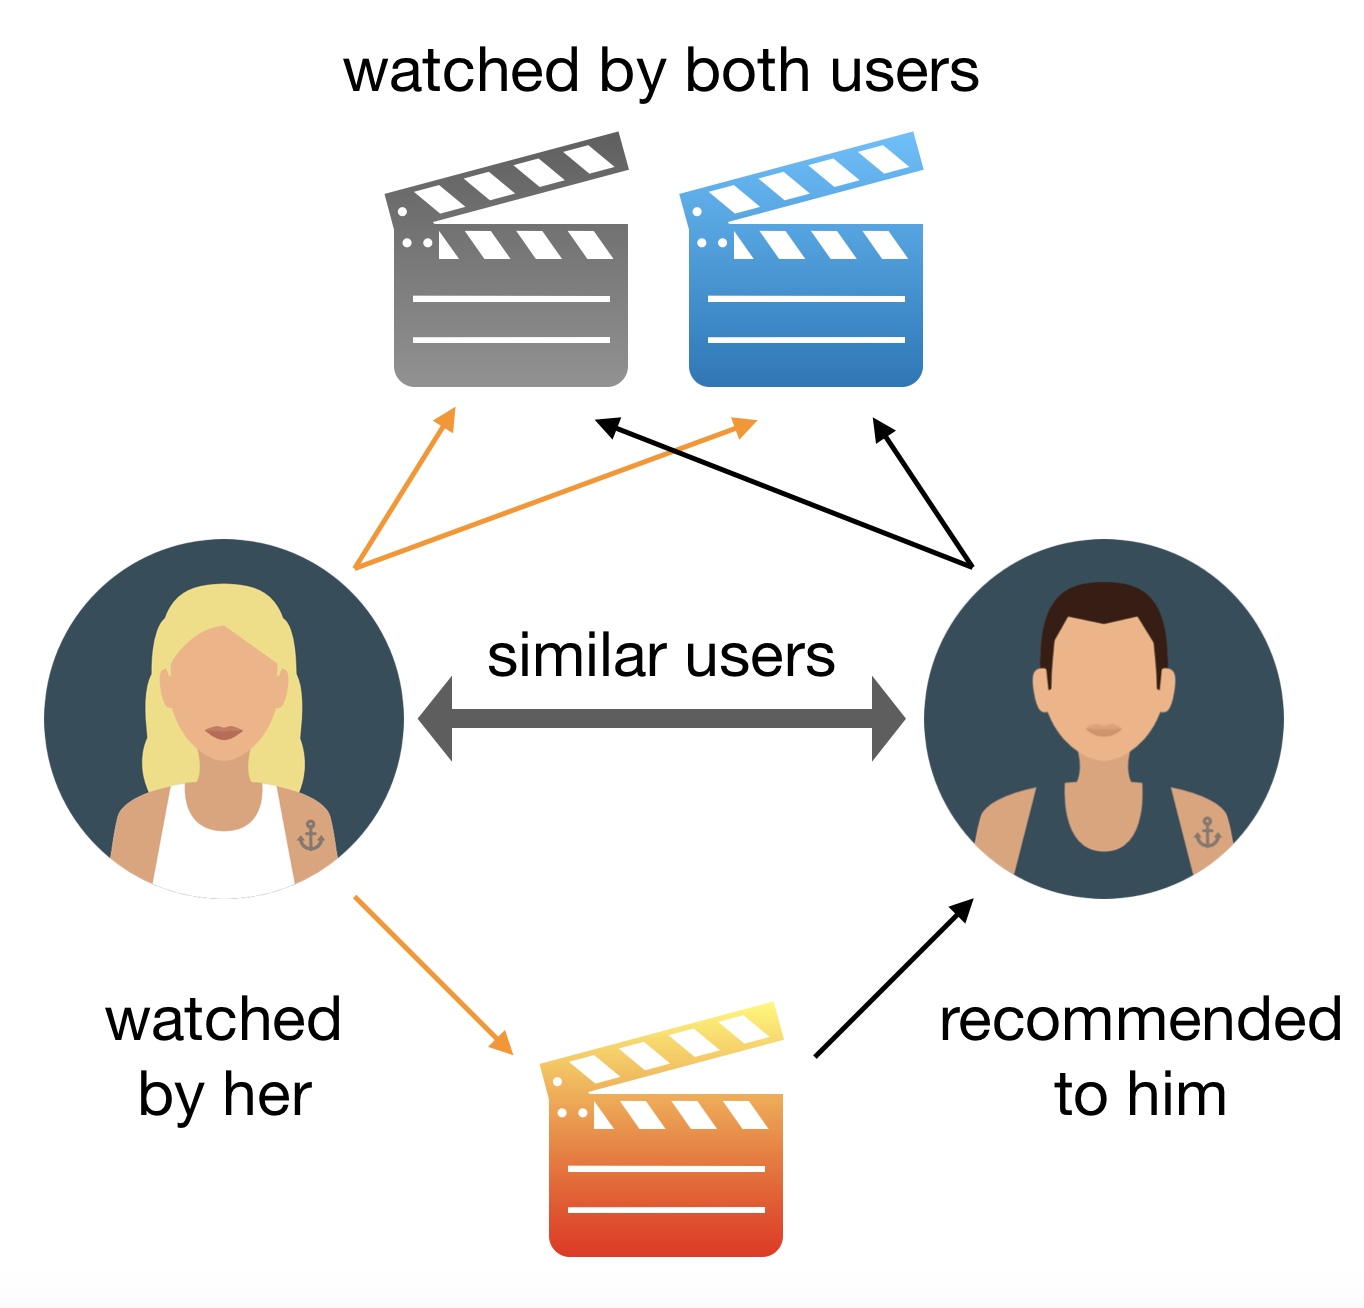
\includegraphics[scale=0.1]{images/cf-idea.png}
\end{center}
\end{column}

\end{columns}

\end{frame}

%--------------------------------------------------

\begin{frame}
\begin{center}
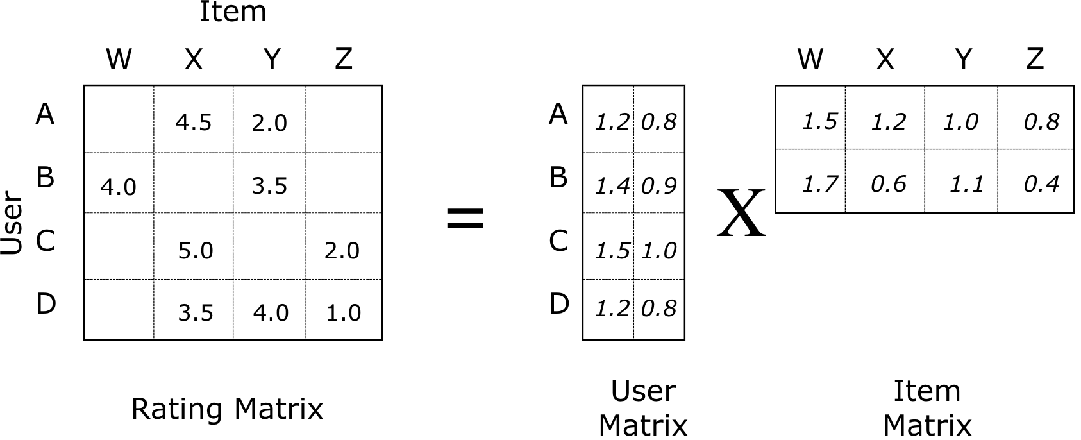
\includegraphics[scale=0.5]{images/SVD.png}
\end{center}
\end{frame}

%--------------------------------------------------

\begin{frame}
\begin{center}
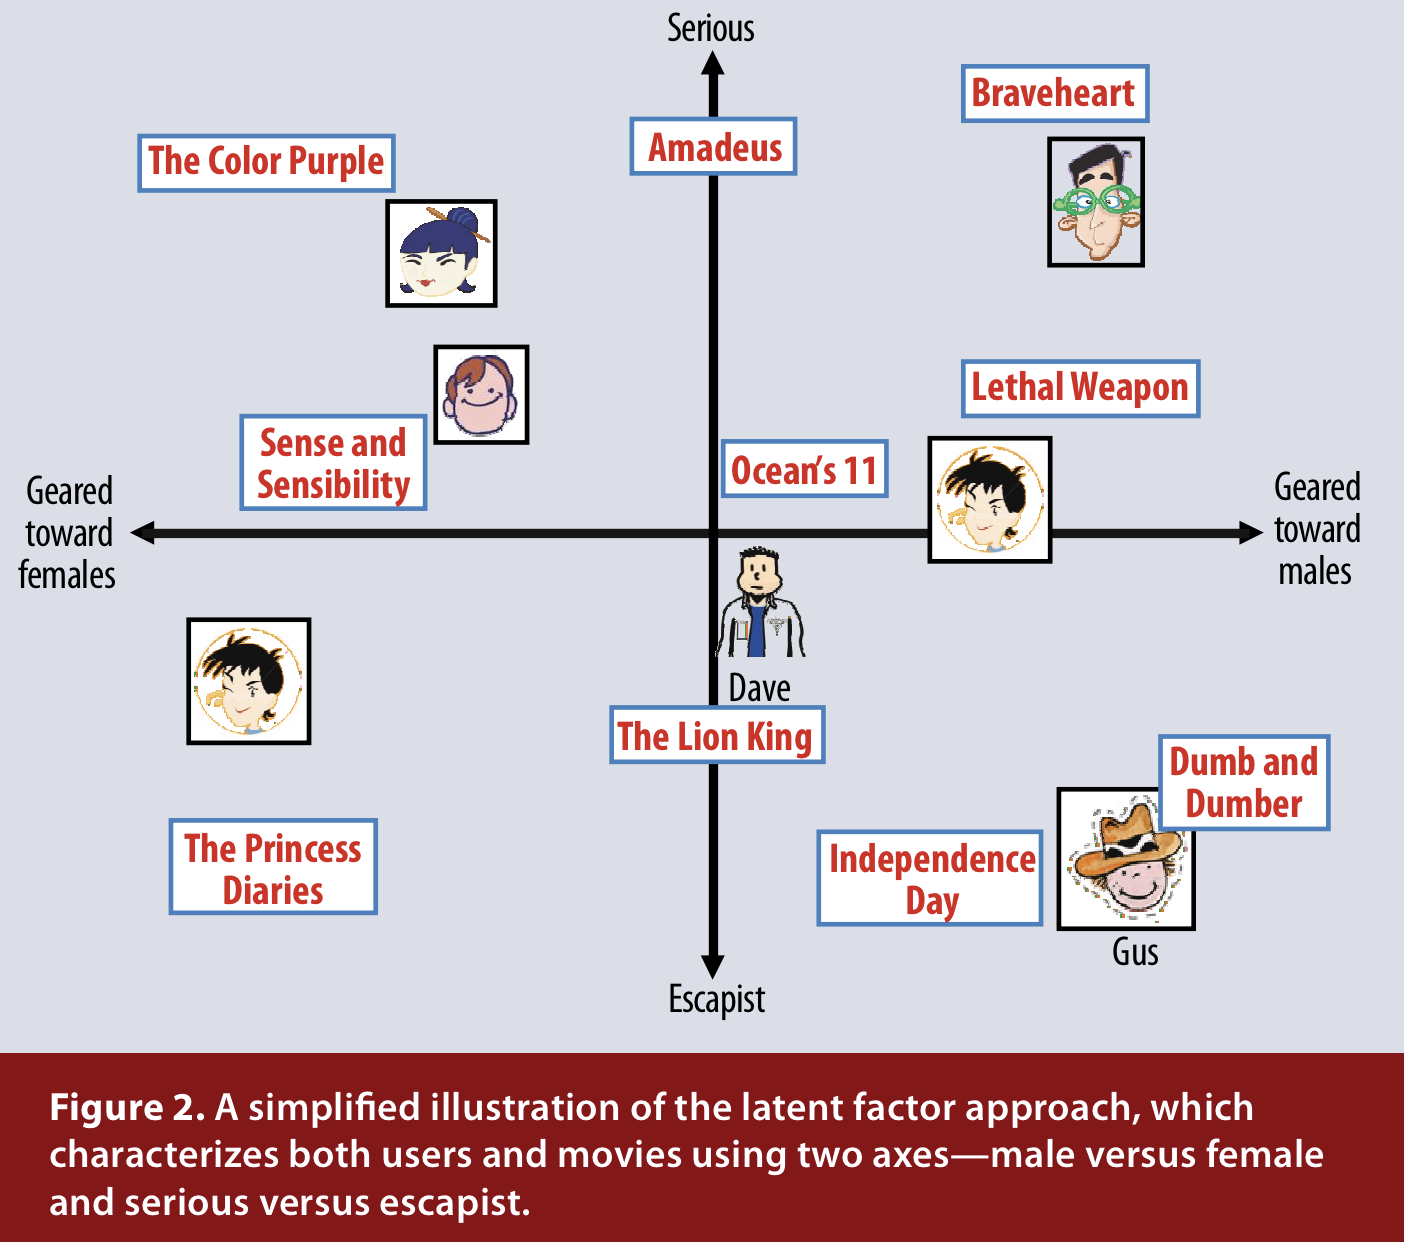
\includegraphics[scale=0.3]{images/latent.png}
\end{center}
\end{frame}

%--------------------------------------------------

\begin{frame}{Простые автоэнкодеры}

SLIM \cite{SLIM} / EASE \cite{EASE}
\[
\hat A = A W,
\]
где
\begin{itemize}
\item $A$ -- матрица интеракций
\item $\hat A$ -- предсказанные интеракции
\item $W_{:,j}$ -- колонка весов агрегации для  $j$ айтема ($W_{ij} \geq 0$ (SLIM), $W_{jj} = 0$).
\end{itemize}

\end{frame}

%--------------------------------------------------

\begin{frame}{Implicit ALS (iALS) \cite{iALS}}
\begin{tcolorbox}[colback=info!5,colframe=info!80,title=]
Давайте обучим модель на implicit feedback, но вместо семплирования implicit негативных примеров - используем вообще все негативные примеры.
\end{tcolorbox}

\[
\mathcal{L} = \sum_{(u, i) \in S} ((q_i^Tp_u) - 1)^2 + \alpha\sum_{u \in U} \sum_{i \in I} (q_i^Tp_u)^2 + \lambda R(P,Q)
\]
\[
R(P,Q) = \sum_{u \in U} (U(i) + \alpha|U|)||p_u||_F + \sum_{i \in I} (I(u) + \alpha|I|)||q_i||_F
\]

При расчете аналитических решений для векторов $p_u$, $q_i$ - значительная часть вычислений является общей. Eë нужно посчитать только один раз и дальше перееиспользовать в рамках одного шага ALS.

\end{frame}

%\begin{frame}{}
%
%\begin{columns}
%
%\begin{column}{0.47\textwidth} 
%\begin{center}
%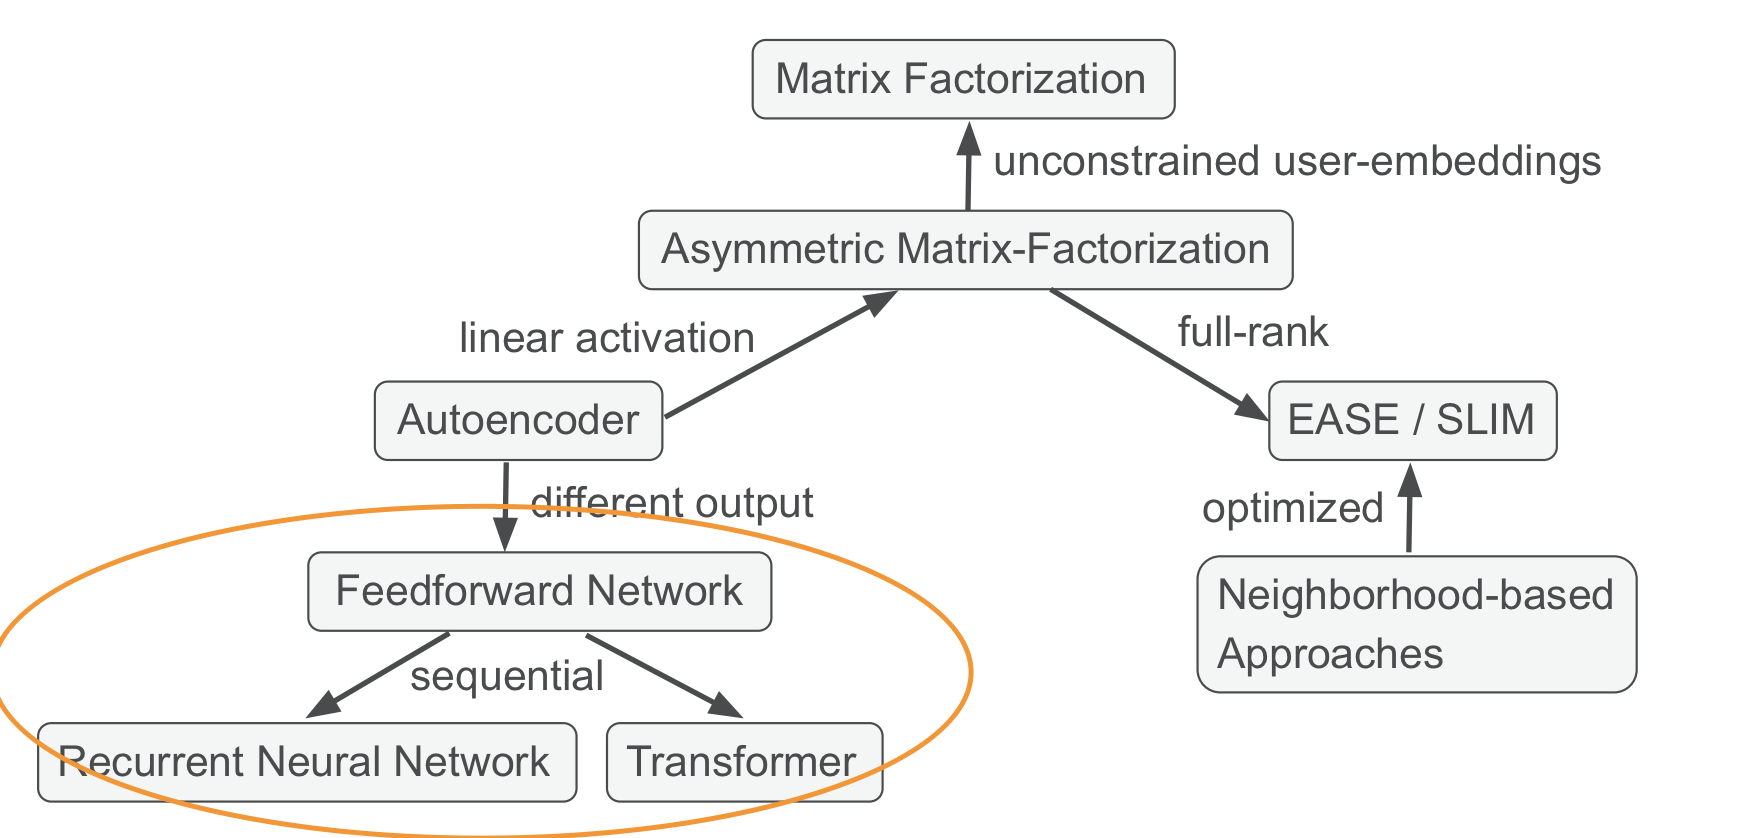
\includegraphics[scale=0.18]{images/relationships.png}
%\end{center}
%\end{column}
%
%\begin{column}{0.47\textwidth}
%\begin{center}
%
\includegraphics[scale=0.15]{images/conspiracy.jpeg}
%\end{center}
%\end{column}
%
%\end{columns}
%
%\end{frame}

\section{Что дальше}

\begin{frame}{Что нужно знать до начала модуля}

\begin{footnotesize}

Базовая математика
\begin{itemize}
\item Операции над векторами и матрицами.
\item Дифференцирование и нахождение минимумов функций.
\item Базовые алгоритмы и структуры данных.
\end{itemize}

Основы машинного обучения
\begin{itemize}
\item Постановка задачи ML, классические алгоритмы.
\item Базовое представление о том как работают современные нейронные сети.
\item Знакомство с рекомендательными системами.
\end{itemize}

Технические скиллы
\begin{itemize}
\item Знание языка python.
\item Знакомство с Docker, умение запустить контейнер.
\item Умение пользоваться git.
\item Небольшой опыт PySpark.
\item Знакомство с архитектурой высоконагруженных сервисов (БД + Big Data).
\end{itemize}

\end{footnotesize}

\end{frame}

\begin{frame}{Программа курса}

\begin{footnotesize}
\begin{tabular}{ c | l | c | c | c }
{\bf Неделя} & {\bf Тема} & {\bf Квиз} & {\bf Семинар} & {\bf Домашка} \\
\hline
0 & Основные подходы рекомендательных систем (вы сейчас на нём!) &  & \checked &  \\
1 & Рекомендательные системы в production & \checked  & \checked &  \\
2 & Нейронные сети для генерации кандидатов & \checked  &  \checked &  \\ 
3 & Нейронные сети для ранжирования & \checked  & \checked & \checked \\
4 & Большие рекомендательные модели & \checked  & \checked & \\
5 & Графовые нейронные сети в рекомендациях & \checked  &  & \\
6 & Разнообразие в рекомендациях & \checked  & \checked & \checked \\
7 & Нерешённые проблемы рекомендательных систем & \checked  & \checked & \\
8 & Uplift моделирование & \checked  & \checked & \checked \\
9 & Reinforcement learning для рекомендаций & \checked  & \checked & 
\end{tabular}
\end{footnotesize}

\end{frame}

\begin{frame}{Оценка $\in [0, 100]$}

\begin{itemize}
\item Идеальное выполнение домашек $25 + 35 = 60$
\item Идеальное выполнение квизов и домашки = $100$
\item Дополнительные баллы можно получить на зачете
\end{itemize}

\end{frame}


\begin{frame}[allowframebreaks]{Литература}
\bibliographystyle{amsalpha}
\bibliography{references.bib}
\end{frame}

\end{document}
